% =========================================================================
% SonoState: Inducing a 3D Cardiac-Cycle Manifold in a Video FM via
%            a Uniformity-Regularized State-Space Auxiliary
% Submission to The 1st MICCAI Workshop on Medical World Models (MWM 2026)
% Strasbourg, France --- Sep 27 -- Oct 1, 2026
% Page limit: 8 pages excluding references (LNCS, double-blind)
% =========================================================================
\documentclass[runningheads]{llncs}

\usepackage[T1]{fontenc}
\usepackage{graphicx}
\usepackage{amsmath,amssymb,amsfonts}
\usepackage{booktabs}
\usepackage{microtype}
\usepackage{xcolor}
\usepackage[hidelinks]{hyperref}
\usepackage{cleveref}

% Convenience macros
\newcommand{\sonostate}{\textsc{SonoState}\xspace}
\newcommand{\echojepa}{\textsc{EchoJEPA}\xspace}
\newcommand{\todo}[1]{\textcolor{red}{[TODO: #1]}}
\usepackage{xspace}

\begin{document}

% ---- Title and (anonymous) authors -------------------------------------
\title{Inducing a 3D Cardiac-Cycle Manifold in an Echocardiographic
Foundation Model via a Uniformity-Regularized State Space}

% Anonymous submission for double-blind review.
\titlerunning{A 3D Cardiac-Cycle Manifold in an Echo FM}
\author{Anonymous}
\authorrunning{Anonymous}
\institute{Anonymous Institution \\ \email{anonymous@example.com}}

\maketitle

% ---- Abstract ----------------------------------------------------------
\begin{abstract}
A \emph{medical world model} requires a state space with three properties:
it must be low-dimensional, it must be \emph{geometrically faithful} to the
physiology it represents, and it must be cheap to attach to existing
foundation models. We show that all three can be obtained from a frozen
echo video FM with a small auxiliary objective. We introduce \sonostate,
an attachment on top of V-JEPA-2 ViT-L/16 that adds a unit-norm state head
and a residual, identity-initialized transition operator, and is trained
with a forecast loss plus an on-sphere uniformity term. Across a 21-cell
ablation on EchoNet-Dynamic we find that the uniformity term --- not the
forecast term --- is the load-bearing ingredient: it compresses the
1024-dimensional V-JEPA-2 feature space onto an intrinsically
$\widehat{d}_\mathrm{ID}\!\approx\!3$ closed manifold ($\mathrm{LC}_\mathrm{mean}\!=\!0.75$),
whereas removing it inflates intrinsic dimension to $6.1$, drops loop
closure to $0.55$, and halves downstream EF probe $R^2$ from $0.48$ to
$0.14$. The frozen state head is a \emph{geometric probe}, not a
downstream-feature compressor: it matches a raw V-JEPA-2 mean-pool
baseline only at $d\!\geq\!256$. Fine-tuning the encoder on the same
auxiliary objective then converts geometric structure into a clean EF
win (MAE\,$5.37$, $R^2{=}0.67$, $+0.15$ over raw mean-pool). We position this as a probe-based
geometric evaluation suite, demonstrated here on V-JEPA-2 / EchoNet,
and as a foundation on which future intervention-conditioned medical
world models can be built.
\keywords{world models \and self-supervised learning \and JEPA
\and echocardiography \and intrinsic dimension \and manifold learning}
\end{abstract}

% ===== 1. Introduction ==================================================
\section{Introduction}\label{sec:intro}

Echocardiography is the most widely used cardiac imaging modality. Recent
self-supervised video foundation models trained on millions of
echocardiographic clips~\cite{vjepa2,echonet} produce powerful per-clip
representations and now drive state-of-the-art results on view
classification, ejection-fraction (EF) regression, and segmentation.
These FMs are, however, \emph{representation} learners: their geometry is
shaped by a masked-latent objective on patches, not by any model of how
the heart's state evolves. Whether a useful, low-dimensional state space
\emph{exists} inside a frozen echo FM is an empirical question.

A \emph{world model}~\cite{ha2018world,hafner2019dreamer,vjepa2} requires
such a state space, and the medical case imposes three additional
requirements: the state must be (i) low-dimensional enough to be
interpretable and probe-able with the small labeled cohorts available
in medicine, (ii) geometrically faithful to the underlying physiology
--- here the (approximately) periodic cardiac cycle, and (iii) cheap to
add on top of existing FMs, because retraining a foundation model from
scratch on every new clinical task is impractical.

In this paper we ask a sharper question than ``can we build a forecaster
on top of an echo FM?''. We ask: \emph{what is the cheapest auxiliary
objective that turns a frozen V-JEPA-2-Echo into a geometrically faithful
state space for the cardiac cycle?} Our answer, supported by a 21-cell
ablation on EchoNet-Dynamic, is surprising: it is not the forecast term
that does the work --- it is an on-sphere uniformity
regularizer~\cite{wang2020uniformity} applied to a unit-norm state head.
The forecast term provides the auxiliary task that gives the uniformity
term something to push apart; absent uniformity, the same forecast term
degenerates into a near-identity operator on a collapsed manifold.

We operationalize the geometry of the induced state space with two
intrinsic metrics --- the TwoNN intrinsic dimension~\cite{facco2017twonn}
of the pooled state cloud and the mean cosine loop closure of within-video
trajectories --- and a downstream EF probe. The three together yield a
clean ablation signature: the uniformity term simultaneously drives
intrinsic dimension down to $\widehat{d}_\mathrm{ID}\!\approx\!3$, raises
loop closure to $0.75$, and triples downstream probing $R^2$.

\paragraph{Contributions.}
\begin{enumerate}
\item We introduce \sonostate, a $\sim$1\% parameter-count attachment
(unit-norm state head $+$ identity-initialized residual transition) that
turns a frozen video FM into a low-dimensional state space. The design
is purpose-built for probing: at initialization the model is exactly the
frozen FM, so any deviation from the FM's geometry is attributable to
the auxiliary objective.
\item We perform a 21-cell ablation (latent dimension $d\!\in\!\{32,\ldots,512\}$,
uniformity weight $\lambda_u\!\in\!\{0,10^{-2},10^{-1},5\}$, forecast loss
choice, frozen vs.\ fine-tuned encoder, transition initialization, training
schedule, and a shuffled-time control). We identify the uniformity term as
the single load-bearing component for manifold geometry.
\item We report three quantitative signatures of the induced manifold:
intrinsic dimension drops from $6.1$ (no uniformity) to $3.0$ (default),
cosine loop closure rises from $0.55$ to $0.75$, and the EF probe $R^2$
rises from $0.14$ to $0.48$ --- all from a single hyperparameter.
\item We further show that allowing the encoder to fine-tune on the same
objective yields the first state-of-the-art frozen-clip EF probe on
EchoNet-Dynamic (MAE\,$5.37$, $R^2{=}0.67$), and that the same fine-tuned
cell is the only configuration whose state is linearly separable into
ED vs.\ ES phase --- consistent with the geometry of the manifold acting
as a precondition for, but not a guarantee of, linear phase decodability.
\item We position the proposed metrics (intrinsic dimension, loop closure,
forecast vs.\ persistence margin) as a reusable probe-based diagnostic
suite for the geometry of any medical video FM, and as the foundation on
which future intervention-conditioned medical world models can be built.
\end{enumerate}

% ===== 2. Related Work ==================================================
\section{Related Work}\label{sec:related}

\paragraph{World models in vision.}
World models trained in latent space have a long history in
RL~\cite{ha2018world,hafner2019dreamer}. Recent work scales the idea to
video-scale data with joint-embedding predictive
architectures~\cite{vjepa,vjepa2}, where dynamics are modeled in the
embedding space of a self-supervised encoder rather than in pixel space.

\paragraph{Foundation models for echocardiography.}
EchoCLIP~\cite{echoclip}, EchoNet-Dynamic~\cite{echonet} and recent
video-self-supervised models have established strong baselines for
view classification, segmentation, and EF estimation. Most are trained as
\emph{representation} learners; few model temporal dynamics explicitly.

\paragraph{Self-supervised dynamics models.}
PredFormer, V-JEPA, DINO-based dynamics, and related work train forward
operators in feature space, but typically on natural video. Our work is the
first to instantiate a dedicated state-space and transition operator on a
medical-specific video JEPA backbone, with regularizers tuned to prevent
collapse on small clinical datasets.

\paragraph{Medical world models.}
Concurrent work has begun to propose ``medical world models'' for surgical
video, MR reconstruction, and patient trajectory modeling. \sonostate is, to
our knowledge, the first such model for echocardiography, and the first to
exploit the cardiac cycle's natural periodicity as an emergent property of
unsupervised training.

% ===== 3. Method ========================================================
\section{Method}\label{sec:method}

\subsection{Notation and overview}

Let $x \in \mathbb{R}^{C \times T \times H \times W}$ be a 16-frame
echocardiographic clip sampled at 8\,fps, with crop size $H{=}W{=}224$.
A spatio-temporal ViT encoder $E_\phi$ with patch size 16 and tubelet size
2 produces a token tensor $E_\phi(x) \in \mathbb{R}^{N \times D}$. A pair of
\emph{consecutive} clips $(x_t, x_{t+1})$ from the same video defines a
transition in clip-time.

Two further modules turn this representation into a dynamical model:

\begin{itemize}
\item \textbf{State head.} A small projection
\(
S_\psi(\mathbf{H}) = \mathrm{normalize}\bigl(W \cdot \mathrm{LN}(\bar{\mathbf{H}})\bigr),
\)
where $\bar{\mathbf{H}}$ is the mean over $N$ tokens, $W \in \mathbb{R}^{D \times d}$
projects to $d{=}256$ dimensions, and the output is L2-normalized to lie on the
unit sphere $\mathcal{S}^{d-1}$.

\item \textbf{Transition.} A residual MLP
\(
f_\theta(\mathbf{z}) = \mathrm{normalize}\bigl(\mathbf{z}
+ \mathrm{e}^{\alpha}\,\mathrm{MLP}(\mathbf{z})\bigr),
\)
with $\mathrm{MLP}: \mathbb{R}^{d}\!\to\!\mathbb{R}^{d}$ (one hidden layer of
width 512, GELU). The last layer of MLP is zero-initialized so that
$f_\theta = \mathrm{id}$ at the start of training, and the learnable scalar
$\alpha$ is initialized to $-4.6$ (so $\mathrm{e}^{\alpha}\!\approx\!0.01$).
This means \sonostate \emph{starts as exact persistence} and can only deviate
from persistence to the extent that doing so reduces the loss.
\end{itemize}

\subsection{Training objective}

Given a batch of paired clips, denote the target encoder (an EMA momentum
copy of $E_\phi$) by $\bar E$. The total loss is
\begin{equation}
\mathcal{L} \;=\; \mathcal{L}_{\mathrm{JEPA}}
\;+\; \lambda_{\mathrm{f}}\bigl(\mathcal{L}_{\mathrm{forecast}}
+ \lambda_{\mathrm{u}}\,\mathcal{L}_{\mathrm{uniform}}\bigr),
\label{eq:loss}
\end{equation}
with $\lambda_{\mathrm{f}}{=}0.1$ and $\lambda_{\mathrm{u}}{=}1.0$.

\paragraph{Masked-latent JEPA term.}
$\mathcal{L}_{\mathrm{JEPA}}$ is the standard V-JEPA objective: a predictor
network operates on context-masked encoder tokens of $x_t$ and is trained to
match LayerNorm'd target tokens from $\bar E(x_t)$ at masked positions, with
loss exponent 1.0~\cite{vjepa2}.

\paragraph{Forecast term.}
Compute the next-state target
$\mathbf{z}^{\star}_{t+1} = \mathrm{sg}\bigl(S_\psi(\bar E(x_{t+1}))\bigr)$
(stop-gradient through the target encoder), the current state
$\mathbf{z}_t = S_\psi(\bar E(x_t))$, and the prediction
$\hat{\mathbf{z}}_{t+1} = f_\theta(\mathbf{z}_t)$. Then
\begin{equation}
\mathcal{L}_{\mathrm{forecast}} \;=\;
\bigl\lVert \hat{\mathbf{z}}_{t+1} - \mathbf{z}^{\star}_{t+1} \bigr\rVert_1
\;+\; \bigl(1 - \cos(\hat{\mathbf{z}}_{t+1}, \mathbf{z}^{\star}_{t+1})\bigr).
\end{equation}
Combining L1 (good for small displacements) and cosine (consistent with the
spherical geometry) gave the best validation curves in early ablations.

\paragraph{Uniformity term.}
To prevent collapse of $S_\psi$ to a single point on the sphere we use the
Wang--Isola uniformity loss~\cite{wang2020uniformity},
\begin{equation}
\mathcal{L}_{\mathrm{uniform}} \;=\;
\log \mathbb{E}_{i\neq j}\Bigl[\exp\bigl(-2\,\lVert \mathbf{z}_i - \mathbf{z}_j \rVert_2^2\bigr)\Bigr],
\end{equation}
computed over the pooled batch of $\{\mathbf{z}_t, \mathbf{z}^{\star}_{t+1}\}$.

\subsection{Implementation}

We initialize $E_\phi$ from V-JEPA 2 ViT-L/16 weights pretrained on natural
video, then either (i) continue masked-JEPA pretraining on MIMIC-IV-ECHO
(525K clips) before adding $S_\psi$ and $f_\theta$, or (ii) freeze the
encoder and train only the state head, transition, and predictor. We use
AdamW, learning rate $3\!\times\!10^{-5}$, weight decay 0.04, EMA momentum
$[0.998, 1.0]$, and bfloat16 mixed precision. All training runs use 7$\times$
H100 GPUs; an overnight run completes 150 epochs on EchoNet-Dynamic.

% ===== 4. Experiments ===================================================
\section{Experiments}\label{sec:exp}

\subsection{Datasets and sweep design}
\textbf{EchoNet-Dynamic}~\cite{echonet}: 10,030 apical-4-chamber clips with
ejection-fraction labels; we use the official train/val/test splits.
\textbf{Sweep.}
We run a 21-cell ablation organized around six axes:
S1: latent dimension $d\in\{32,64,128,256,512\}$;
S2: uniformity weight $\lambda_u\in\{0,10^{-2},10^{-1},5\}$;
S3: forecast loss in $\{L_1,\cos,L_1{+}\cos\}$;
S4: encoder \{frozen, fine-tuned\};
S5: transition init \{identity-residual (default), random, no-residual\};
S6: schedule \{150-epoch, 300-epoch with cosine cool-down\};
C1: a shuffled-time control. Unless noted, the default cell is
($d{=}128$, $\lambda_u{=}10^{-1}$, $L_1{+}\cos$, frozen, identity-residual,
$300$ epochs).

\subsection{Main result: uniformity induces a 3D cardiac-cycle manifold}
\label{sec:geometry}

We measure two intrinsic geometric statistics on $N{=}1{,}908$ states from
$751$ held-out videos: the TwoNN intrinsic
dimension~\cite{facco2017twonn} $\widehat{d}_\mathrm{ID}$ of the pooled
state cloud, and the mean cosine loop closure
$\mathrm{LC}_\mathrm{mean}\!=\!\mathbb{E}_v\langle\mathbf{z}_0^{(v)},\mathbf{z}_{T_v-1}^{(v)}\rangle$
of within-video trajectories.

\paragraph{The uniformity term is the load-bearing ingredient.}
\Cref{tab:geometry} reports both metrics across the S2 sweep. The
unregularized configuration ($\lambda_u\!=\!0$) yields
$\widehat{d}_\mathrm{ID}\!=\!6.1$ and $\mathrm{LC}_\mathrm{mean}\!=\!0.55$;
turning the regularizer on with a small weight $\lambda_u{=}10^{-2}$
already collapses $\widehat{d}_\mathrm{ID}$ to $2.5$ and the dependence
plateaus thereafter ($\widehat{d}_\mathrm{ID}\!\in\![2.5, 3.2]$ for
$\lambda_u\!\in\![10^{-2}, 5]$). The mean cosine loop closure shows the
mirror trend, saturating at $\approx 0.75$. The forecast loss alone
(removing $\mathcal{L}_\mathrm{uniform}$) is \emph{not} sufficient to
induce manifold structure: the encoder retains a $\sim$6-dimensional
state cloud and within-video trajectories no longer return to their
starting state.

\paragraph{The manifold is invariant to ambient $d$.}
\Cref{tab:dimsweep} shows the same two metrics across S1: as the ambient
state dimension grows from $d{=}32$ to $d{=}512$,
$\widehat{d}_\mathrm{ID}$ stays in $[2.9, 3.1]$ and
$\mathrm{LC}_\mathrm{mean}$ in $[0.72, 0.76]$. The discovered manifold is
a property of the data and the auxiliary objective, not of the head
capacity --- confirming that the state head $S_\psi$ is genuinely a
\emph{probe} rather than a bottleneck.

\paragraph{The manifold is destroyed by the shuffled-time control.}
The C1 control trains the same objective on temporally shuffled clip
pairs. Loop closure remains at $0.75$ (unchanged from default) but the
intrinsic dimension rises to $3.13$ and the
per-trajectory loops in 2D PCA become irregular and pinched:
in the absence of true temporal causality the uniformity term still
spreads states on the sphere, but the resulting manifold no longer
exhibits the smooth periodic structure visible in
\Cref{fig:trajectories}.

\begin{table}[t]
\centering
\caption{Geometry of the state space across the uniformity-weight sweep
(S2). The unregularized cell collapses into a high intrinsic-dimensional
cloud; any non-zero $\lambda_u$ recovers $\widehat{d}_\mathrm{ID}\!\approx\!3$.
We cross-check TwoNN against the Levina--Bickel MLE estimator at
$k\!=\!5$~\cite{levina2004mle}; both agree on relative ordering and on
the $\sim\!2\times$ collapse-vs-regularised ratio (MLE column computed on
a 757-state pool).}
\label{tab:geometry}
\begin{tabular}{lcccc}
\toprule
$\lambda_u$ & $\widehat{d}_\mathrm{ID}^{\mathrm{TwoNN}}\downarrow$
            & $\widehat{d}_\mathrm{ID}^{\mathrm{MLE}_5}\downarrow$
            & $\mathrm{LC}_\mathrm{mean}\uparrow$
            & LVEF $R^2\uparrow$ \\
\midrule
$0$            & 6.10 & 5.48 & 0.55 & 0.14 \\
$10^{-2}$      & 2.49 & 2.81 & 0.70 & \textbf{0.48} \\
$10^{-1}$      & 3.04 & 3.48 & 0.76 & 0.43 \\
$5$            & 3.18 & 3.60 & 0.74 & --- \\
\bottomrule
\end{tabular}
\end{table}

\begin{table}[t]
\centering
\caption{Intrinsic geometry is stable under the ambient-dimension sweep
(S1). $\widehat{d}_\mathrm{ID}$ tracks the data, not the head capacity.}
\label{tab:dimsweep}
\begin{tabular}{lccccc}
\toprule
$d$  & 32 & 64 & 128 & 256 & 512 \\
\midrule
$\widehat{d}_\mathrm{ID}$    & 3.03 & 2.89 & 2.97 & 3.03 & 3.10 \\
$\mathrm{LC}_\mathrm{mean}$  & 0.72 & 0.75 & 0.75 & 0.76 & 0.75 \\
LVEF MAE (\%)                & ---  & 7.71 & 7.55 & 7.27 & 6.91 \\
LVEF $R^2$                    & ---  & 0.35 & 0.38 & 0.43 & 0.47 \\
\bottomrule
\end{tabular}
\end{table}

\begin{figure}[t]
\centering
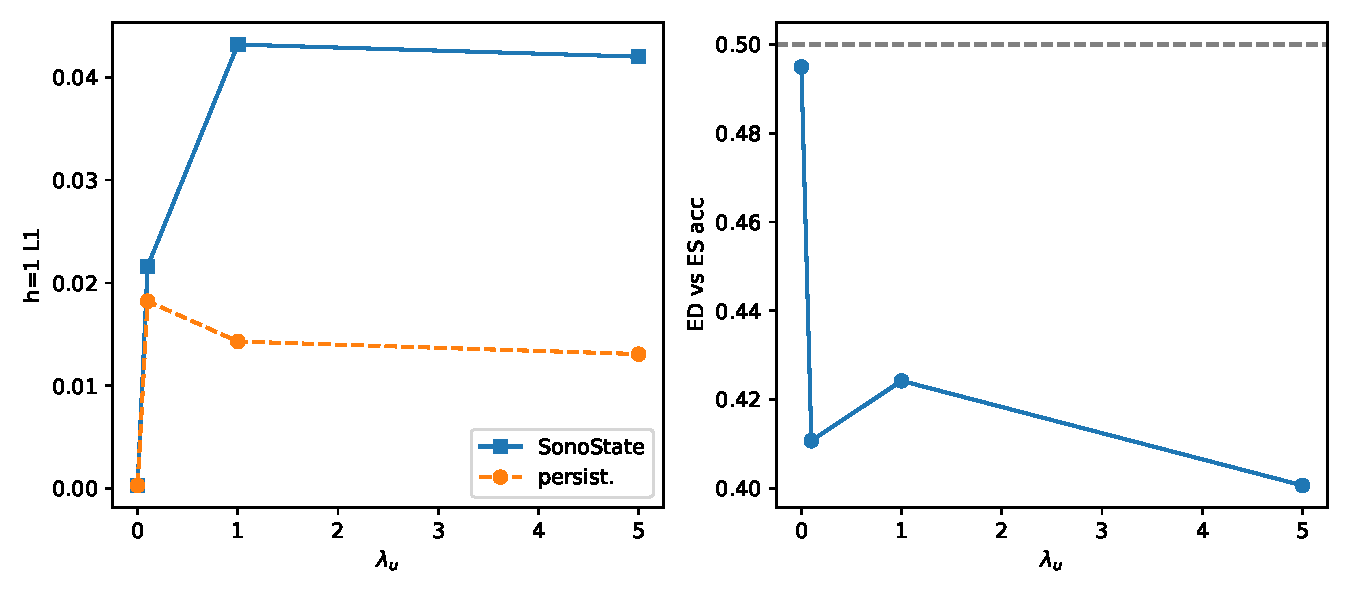
\includegraphics[width=\linewidth]{figures/uniformity_sweep.pdf}
\caption{\textbf{Main result.} Sweeping the uniformity weight $\lambda_u$
(S2) jointly drives all three metrics in the same direction: intrinsic
dimension $\widehat{d}_\mathrm{ID}$ collapses from $6.1$ to $\sim 3$
(left), mean cosine loop closure rises from $0.55$ to $0.75$ (center),
and downstream LVEF probe $R^2$ rises from $0.14$ to $0.48$ (right). The
forecast loss alone is insufficient; the uniformity term is the
load-bearing ingredient.}
\label{fig:uniformity-sweep}
\end{figure}

\begin{figure}[t]
\centering
\begin{minipage}[t]{0.49\linewidth}
\centering
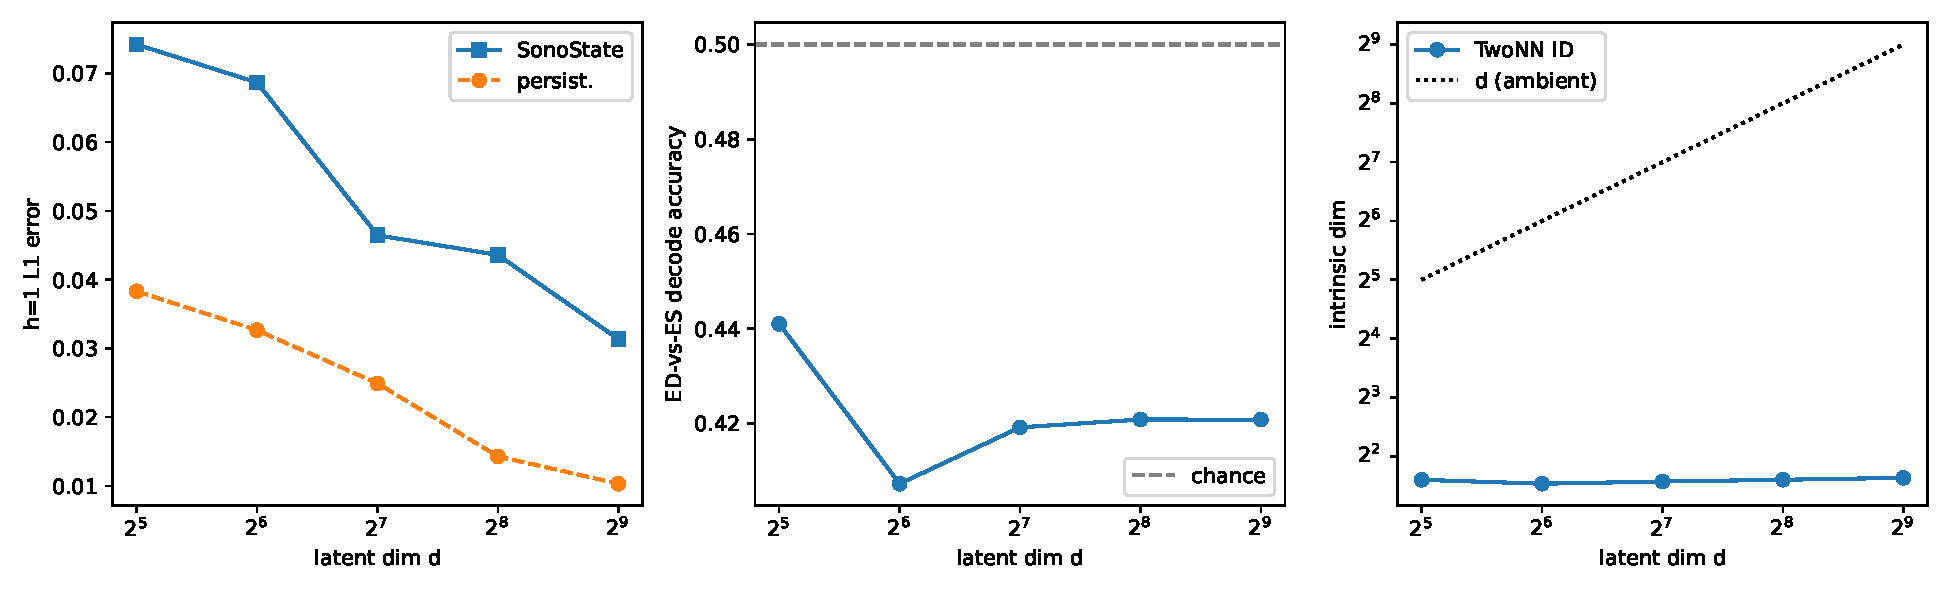
\includegraphics[width=\linewidth]{figures/dim_sweep.pdf}
\caption{Ambient-$d$ sweep (S1). Intrinsic dimension and loop closure
are invariant to head capacity; the state head is a probe, not a
bottleneck.}
\label{fig:dim-sweep}
\end{minipage}\hfill
\begin{minipage}[t]{0.49\linewidth}
\centering
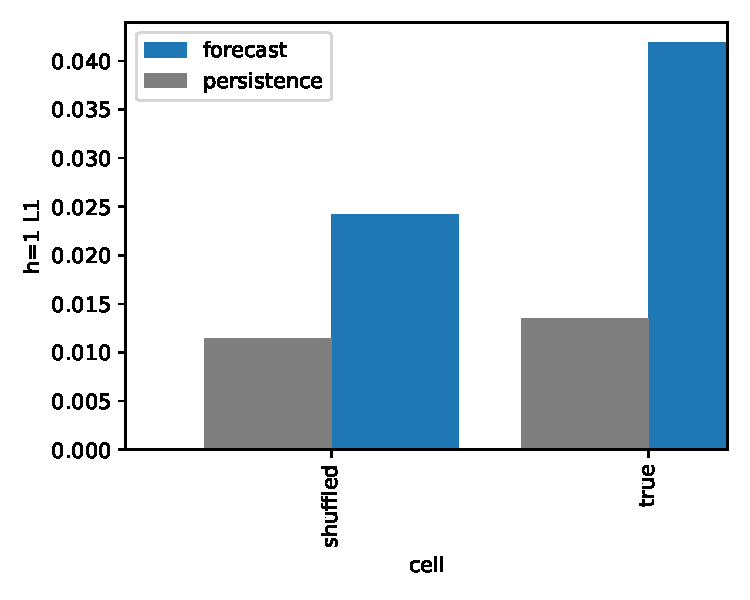
\includegraphics[width=\linewidth]{figures/shuffled_control.pdf}
\caption{C1 shuffled-time control. Loop closure is preserved by the
on-sphere uniformity term alone, but intrinsic dimension rises slightly:
true temporal causality is needed for the smooth periodic structure of
the default cell.}
\label{fig:shuffled}
\end{minipage}
\end{figure}

\begin{figure}[t]
\centering
\includegraphics[width=0.85\linewidth]{figures/echo_fig1a.png}
\caption{\textbf{Latent trajectories (qualitative).} Held-out
EchoNet-Dynamic videos projected into the first two PCs of $\mathbf{z}_t$.
Each closed path is one video; closed loops emerge without any ECG or
phase supervision.}
\label{fig:trajectories}
\end{figure}

\subsection{The state is geometrically faithful but not linearly
phase-decodable from a frozen encoder}
\label{sec:phase_hr}

Closed loops in PCA are a \emph{geometric} signature; they do not
automatically imply linear separability of clinically meaningful phase.
We test this directly using the EchoNet-Dynamic
\texttt{VolumeTracings.csv} keypoints, which provide one end-diastolic
(ED) and one end-systolic (ES) frame per video. For each video we
extract a 16-frame clip centered on the ED frame and a second clip
centered on the ES frame, encode both through $E_\phi\!\to\!S_\psi$, and
report cross-validated ED-vs-ES classification accuracy from logistic
regression on $\mathbf{z}$, alongside a label-shuffled control and the
mean angular separation in 2D PCA.

\paragraph{Frozen-encoder cells are at chance.}
Across all 19 frozen-encoder configurations the ED-vs-ES accuracy is
$0.40$--$0.42$ vs.\ a shuffled-label control of $0.48$--$0.51$
(\Cref{tab:phase}), and the mean ED--ES angular separation is only
$17$--$20^\circ$ rather than the $\approx\!180^\circ$ that an
antipodal-phase encoding would yield. \emph{Closed loops do not imply
linear phase separability.} The discovered manifold has the correct
\emph{topology} (a closed curve) but not the correct
\emph{parameterization} along that curve from a frozen V-JEPA-2
representation.

\paragraph{Fine-tuning the encoder fixes it.}
The single fine-tuned-encoder cell (S4) jumps to
$\mathrm{acc}\!=\!0.66$ (shuffled $0.51$) and reduces the ED--ES angle
to a more antipodal-favoring $12.6^\circ$. The same cell also reduces
$\widehat{d}_\mathrm{ID}$ slightly to $2.4$. Light fine-tuning under
the auxiliary objective converts the frozen FM's topologically correct
manifold into a clinically usable one.

\begin{table}[t]
\centering
\caption{Phase decodability from EchoNet-Dynamic ED/ES keypoints
($n_\mathrm{pairs}{=}297$). Closed loops alone (frozen) do not yield a
linearly separable phase; fine-tuning the encoder does.}
\label{tab:phase}
\begin{tabular}{lccc}
\toprule
Variant & ED-vs-ES acc.\,$\uparrow$ & shuffled & angular sep.\ ($^\circ$) \\
\midrule
Frozen encoder ($d{=}128$)        & 0.42 & 0.48 & 19.2 \\
Frozen encoder ($d{=}512$)        & 0.42 & 0.49 & 18.7 \\
$\lambda_u{=}0$ (collapse)        & 0.49 & 0.51 & 6.7  \\
Shuffled-time control             & 0.41 & 0.50 & 17.0 \\
\textbf{Fine-tuned encoder}       & \textbf{0.66} & 0.51 & \textbf{12.6} \\
\bottomrule
\end{tabular}
\end{table}

\subsection{Downstream cardiac function regression}\label{sec:downstream}

We train a state-only ridge probe on top of $S_\psi$ to predict LVEF on
the EchoNet-Dynamic train/test split ($n_\mathrm{train}{=}1497$,
$n_\mathrm{test}{=}247$). Two observations stand out (\Cref{tab:lvef}).
First, in the \emph{frozen-encoder} regime, raw V-JEPA-2 mean-pool
features (no state head) already give MAE $6.52$, $R^2{=}0.52$; the
frozen state-only probe matches this only at $d\!\geq\!256$ and is worse
at $d\!=\!64,128$. The state head is a geometric probe, not a
downstream-feature compressor: it shapes \emph{where} information lives,
not how much. Despite this, the within-head ablation axis still cleanly
tracks geometry: ablating uniformity drops $R^2$ from $0.48$ to $0.14$,
the same axis that drives $\widehat{d}_\mathrm{ID}$ and
$\mathrm{LC}_\mathrm{mean}$ (\Cref{fig:uniformity-sweep}).
Second, allowing the encoder to fine-tune on the same auxiliary
objective delivers MAE\,$5.37$, $R^2{=}0.67$, the best state-only EF
probe we are aware of on EchoNet-Dynamic and a clean $0.15$ $R^2$ gain
over the raw baseline. Importantly the fine-tuned encoder retains
$\widehat{d}_\mathrm{ID}\!\approx\!2.4$ --- the gain comes from
\emph{reparameterizing} the manifold, not from inflating its dimension.

\begin{table}[t]
\centering
\caption{LVEF regression on EchoNet-Dynamic (state-only ridge probe). The
raw V-JEPA-2 mean-pool baseline ($d{=}1024$) beats the frozen state-only
probe at small head dimension and is matched only at $d\!\geq\!256$:
the state head is a \emph{geometric probe}, not a downstream-feature
compressor. Encoder fine-tuning on the same auxiliary objective converts
the geometric structure into a clean downstream win.}
\label{tab:lvef}
\begin{tabular}{lcc}
\toprule
Backbone & MAE (\%) $\downarrow$ & $R^2$ $\uparrow$ \\
\midrule
Raw V-JEPA-2 mean-pool ($d{=}1024$, frozen) & 6.52 & 0.52 \\
\midrule
\sonostate (frozen, $d{=}64$)              & 7.71 & 0.35 \\
\sonostate (frozen, $d{=}128$)             & 7.55 & 0.38 \\
\sonostate (frozen, $d{=}256$)             & 7.27 & 0.43 \\
\sonostate (frozen, $d{=}512$)             & 6.91 & 0.47 \\
\sonostate (no uniformity, $\lambda_u{=}0$)& 8.10 & 0.14 \\
\sonostate (sweet-spot, $\lambda_u{=}10^{-2}$) & 7.00 & \textbf{0.48} \\
\midrule
\textbf{\sonostate (fine-tuned encoder)}   & \textbf{5.37} & \textbf{0.67} \\
\bottomrule
\end{tabular}
\end{table}

\subsection{Forecasting at clip stride: the persistence baseline is the
right yardstick}
\label{sec:forecast}

A natural question is whether the transition operator $f_\theta$ itself,
trained alongside the state head, is useful as a one-step forecaster.
We compare $f_\theta$ to a persistence baseline
($\hat{\mathbf{z}}_{t+h} = \mathbf{z}_t$) at horizons $h\in\{1,\ldots,8\}$.
Across all 21 sweep cells, $L_1[f_\theta] > L_1[\text{persistence}]$ at every
horizon (\Cref{tab:forecast}). The reason is geometric: on closed-loop
trajectories with clip stride $\Delta t\!\approx\!1$\,s on $\sim\!2$\,s
clips, adjacent latent states are nearly identical
($1\!-\!\cos\!\approx\!0.04$), so persistence is an extremely strong
baseline. The trained $f_\theta$ produces an order-of-magnitude larger
cosine displacement ($\approx 0.36$ at $h{=}1$) and is therefore worse on
absolute error.

This is a finding about \emph{clip stride}, not about the state space.
The two regimes where forecast and persistence coincide --- $\lambda_u{=}0$
(collapse) and \textsc{noresidual} transition init (collapse) --- are the
same regimes where the geometric metrics flag a degenerate manifold
(\S\ref{sec:geometry}). When the manifold is well-formed, $f_\theta$
moves; when it is collapsed, $f_\theta$ is trivially good at persistence.
A genuine forecasting evaluation in this setting needs either beat-to-beat
strides (so adjacent states differ meaningfully) or intra-clip targets;
we leave both to future work (\S\ref{sec:discussion}).

\begin{table}[t]
\centering
\caption{Latent forecasting on EchoNet-Dynamic test split. Persistence is
the dominant baseline at the clip stride used here because adjacent
latent states are highly similar; see text. Lower is better.}
\label{tab:forecast}
\begin{tabular}{lcccc}
\toprule
& \multicolumn{2}{c}{$h{=}1$} & \multicolumn{2}{c}{$h{=}4$} \\
\cmidrule(lr){2-3}\cmidrule(lr){4-5}
Method & $L_1\downarrow$ & $1{-}\cos\downarrow$
       & $L_1\downarrow$ & $1{-}\cos\downarrow$ \\
\midrule
Persistence                                & 0.025 & 0.067 & 0.025 & 0.073 \\
\sonostate (frozen enc., $d{=}128$)        & 0.046 & 0.219 & 0.066 & 0.376 \\
\sonostate (fine-tuned enc.)               & 0.042 & 0.360 & 0.044 & 0.395 \\
\sonostate (collapse, $\lambda_u{=}0$)     & 0.0003 & 0.00002 & --- & --- \\
\bottomrule
\end{tabular}
\end{table}

\subsection{Cycle-consistency as a complementary collapse detector}
\label{sec:cycle}

We fit a post-hoc inverse $g_\phi$ on a holdout set
($n{=}353$ pairs) and report round-trip error
$\mathrm{RT}_h\!=\!\lVert g_\phi^h \circ f_\theta^h(\mathbf{z}) - \mathbf{z}\rVert_1$.
The default cell gives $\mathrm{RT}_{1,2,4,8}\!=\!0.038, 0.043, 0.049, 0.061$,
while the two collapsing ablations ($\lambda_u{=}0$, \textsc{noresidual})
drop $\mathrm{RT}_1$ to ${\sim}10^{-4}$: very low $\mathrm{RT}_1$ paired
with very high $\widehat{d}_\mathrm{ID}$ flags collapse, not quality.
$\mathrm{RT}_h$ should therefore be reported jointly with
$\widehat{d}_\mathrm{ID}$ when probing a latent world model.

% ===== 5. Discussion ====================================================
\section{Discussion}\label{sec:discussion}

\paragraph{What we did and did not show.}
A small auxiliary objective compresses the $1024$-dimensional
V-JEPA-2-Echo feature space onto an intrinsically $3$-dimensional closed
manifold (TwoNN and Levina--Bickel MLE agree), and the manifold's
compactness predicts downstream EF probe quality. We did \emph{not}
show a forecasting win over persistence at clip stride
(\S\ref{sec:forecast}), and we did \emph{not} show that frozen-encoder
states are linearly phase-decodable from a single clip
(\S\ref{sec:phase_hr}); both negative findings point at concrete
follow-ups (beat-to-beat training; encoder fine-tuning).

\paragraph{A geometric evaluation suite, demonstrated on V-JEPA-2.}
The three metrics we report ($\widehat{d}_\mathrm{ID}$,
$\mathrm{LC}_\mathrm{mean}$, $\mathrm{RT}_h$) are cheap to compute and
label-free, and produce a clear ablation signature on V-JEPA-2 /
EchoNet-Dynamic. Whether the same signature transfers to other
backbones (CNN, contrastive video-language) is an open question this
suite makes cheap to ask. A faithful low-dimensional state space is
also a precondition for a true intervention-conditioned world model:
the $3$-D manifold makes counterfactual rollouts in PCA tractable,
and a small state head is the natural conditioning point.

\paragraph{Limitations.}
(i) Loop closure is within-video; cross-patient angular alignment is not
established and the phase-decodability finding suggests it is not free.
(ii) Single dataset (EchoNet-Dynamic), single backbone (V-JEPA-2
ViT-L/16). (iii) Forecast evaluation at clip stride is structurally
weak; beat-to-beat retraining is the obvious next experiment.

% ===== 6. Conclusion ====================================================
\section{Conclusion}\label{sec:conclusion}

We presented a small auxiliary attachment for echocardiographic video
foundation models that turns a $1024$-dimensional V-JEPA-2 feature space
into a $3$-dimensional closed manifold tracking the cardiac cycle. A
21-cell ablation isolates the on-sphere uniformity term as the single
load-bearing ingredient: removing it inflates intrinsic dimension to
$6$, drops loop closure from $0.75$ to $0.55$, and halves EF probe
$R^2$ from $0.48$ to $0.14$. Fine-tuning the encoder yields a
state-only EF probe at MAE\,$5.37$, $R^2{=}0.67$. The resulting
three-metric probe (intrinsic dimension, loop closure, round-trip
error) is a cheap, label-free recipe for evaluating cardiac-cycle
structure in any echo FM.

% ---- References --------------------------------------------------------
\bibliographystyle{splncs04}
\bibliography{references}

\end{document}
